\subsubsection{Visualizing CNN Features with t-SNE}\label{sec:visualizing-cnn-features-with-t-sne}

We already said that a CNN transforms an image $I$ into a latent feature vector:
\begin{equation*}
    \mathbf{z} = \mathrm{FEN}(I)
\end{equation*}
Not the question is: \emph{\textbf{does this learned feature space organize images in a more meaningful way than raw pixel space?}} To answer this question, we can repeat the t-SNE experiment we did on \autopageref{sec:cifar-10-and-t-sne-interpretation}, but this time using \textbf{CNN latent vectors instead of raw pixels}.

\highspace
We use a pretrained architecture called AlexNet, which was trained on the ImageNet dataset, and consider its \textbf{4096-dimensional latent representation} right before the classifier. Thus, for an image $I$, we compute its latent representation:
\begin{equation*}
    \mathrm{FEN}(I) \in \mathbb{R}^{4096}
\end{equation*}

\highspace
\begin{figure}[!htp]
\centering
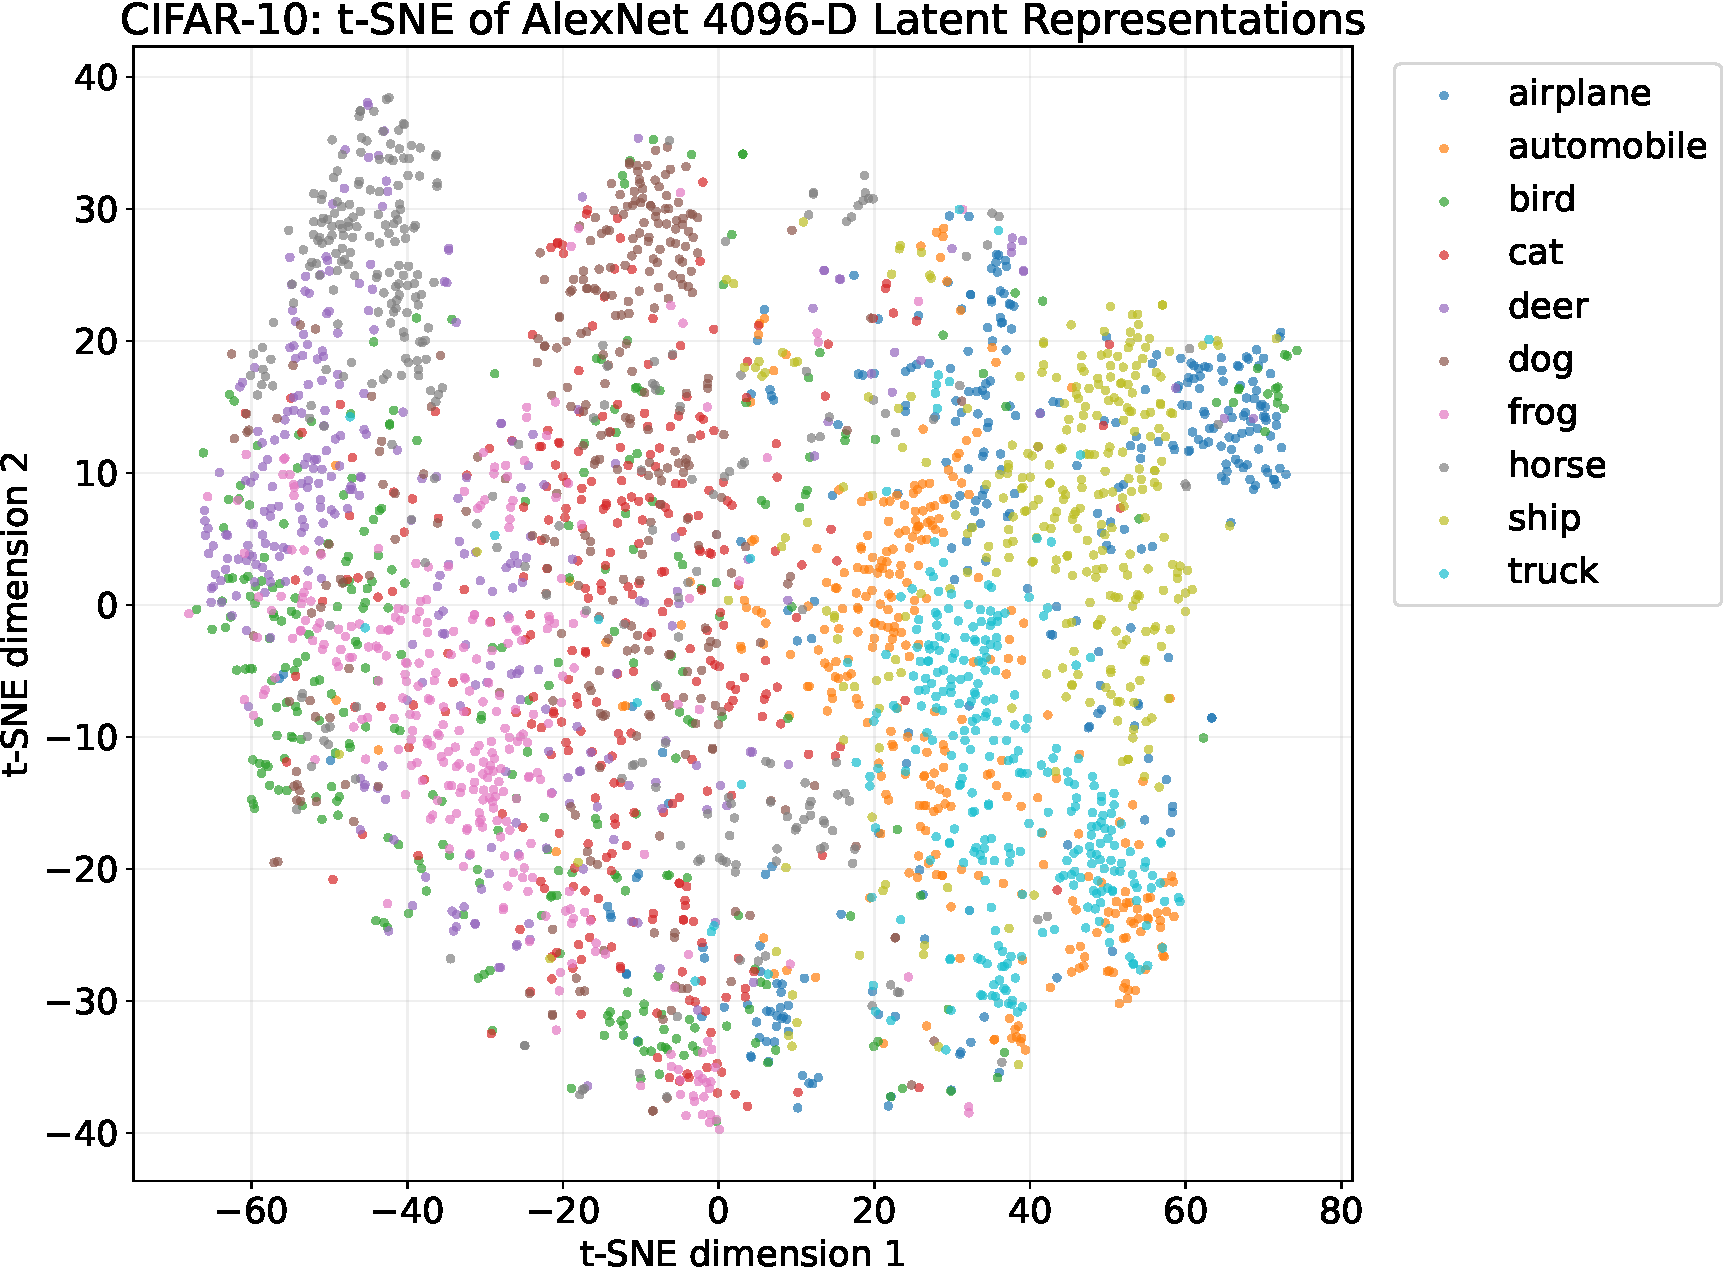
\includegraphics[width=\textwidth]{img/cnn/cifar10-alexnet-tsne.pdf}
\caption{\textbf{t-SNE visualization of AlexNet latent representations on CIFAR-10.} Each CIFAR-10 image is mapped by a pretrained AlexNet to its $4096$-dimensional latent representation immediately before the final classifier, and t-SNE projects these feature vectors into two dimensions. Colors indicate the ground-truth classes. Despite some overlap, semantically related images tend to occupy similar regions of the latent space, showing that distances between learned CNN features are more meaningful than distances between raw pixels.}
\label{fig:cifar10-alexnet-tsne}
\end{figure}

\newpage

\noindent
\textcolor{Green3}{\faIcon{question-circle} \textbf{What do we expect from a good latent space?}} Suppose two images are semantically similar, for example two different images of the same type of object. Even if their pixel values differ considerably because of position, illumination, background, etc., the CNN may produce similar high-level representations for both images:
\begin{equation*}
    \mathrm{FEN}\left(I_1\right) \approx \mathrm{FEN}\left(I_2\right)
\end{equation*}
Therefore their latent-space distance becomes small:
\begin{equation*}
    \left\| \mathrm{FEN}\left(I_1\right) - \mathrm{FEN}\left(I_2\right) \right\| \approx 0
\end{equation*}
That means \hl{semantically related images tend to appear close together in the t-SNE visualization.} Indeed, on \autoref{fig:cifar10-alexnet-tsne}, we see that images of the same class tend to cluster together, and semantically related classes (e.g., cats and dogs) are also close to each other. This is in stark contrast to the t-SNE visualization of raw pixels on \autoref{fig:cifar10-raw-pixels-tsne} (\autopageref{fig:cifar10-raw-pixels-tsne}), where images of different classes are heavily mixed.

\highspace
\begin{takeawaysbox}
    CNNs transform raw images into learned latent vectors in which semantic similarity is better represented. AlexNet, for example, produces a $4096$-dimensional feature vector before the classifier, and image similarity can be measured as
    \begin{equation*}
        d\left(I_1,I_2\right)=\left\|\mathrm{FEN}\left(I_1\right)-\mathrm{FEN}\left(I_2\right)\right\|_{2}
    \end{equation*}
    When these vectors are visualized with t-SNE, semantically similar images tend to lie close together. The key improvement is therefore \textbf{not a different distance metric, but a better representation space}.
\end{takeawaysbox}